% Options for packages loaded elsewhere
% Options for packages loaded elsewhere
\PassOptionsToPackage{unicode}{hyperref}
\PassOptionsToPackage{hyphens}{url}
\PassOptionsToPackage{dvipsnames,svgnames,x11names}{xcolor}
%
\documentclass[
  letterpaper,
  DIV=11,
  numbers=noendperiod]{scrartcl}
\usepackage{xcolor}
\usepackage{amsmath,amssymb}
\setcounter{secnumdepth}{-\maxdimen} % remove section numbering
\usepackage{iftex}
\ifPDFTeX
  \usepackage[T1]{fontenc}
  \usepackage[utf8]{inputenc}
  \usepackage{textcomp} % provide euro and other symbols
\else % if luatex or xetex
  \usepackage{unicode-math} % this also loads fontspec
  \defaultfontfeatures{Scale=MatchLowercase}
  \defaultfontfeatures[\rmfamily]{Ligatures=TeX,Scale=1}
\fi
\usepackage{lmodern}
\ifPDFTeX\else
  % xetex/luatex font selection
\fi
% Use upquote if available, for straight quotes in verbatim environments
\IfFileExists{upquote.sty}{\usepackage{upquote}}{}
\IfFileExists{microtype.sty}{% use microtype if available
  \usepackage[]{microtype}
  \UseMicrotypeSet[protrusion]{basicmath} % disable protrusion for tt fonts
}{}
\makeatletter
\@ifundefined{KOMAClassName}{% if non-KOMA class
  \IfFileExists{parskip.sty}{%
    \usepackage{parskip}
  }{% else
    \setlength{\parindent}{0pt}
    \setlength{\parskip}{6pt plus 2pt minus 1pt}}
}{% if KOMA class
  \KOMAoptions{parskip=half}}
\makeatother
% Make \paragraph and \subparagraph free-standing
\makeatletter
\ifx\paragraph\undefined\else
  \let\oldparagraph\paragraph
  \renewcommand{\paragraph}{
    \@ifstar
      \xxxParagraphStar
      \xxxParagraphNoStar
  }
  \newcommand{\xxxParagraphStar}[1]{\oldparagraph*{#1}\mbox{}}
  \newcommand{\xxxParagraphNoStar}[1]{\oldparagraph{#1}\mbox{}}
\fi
\ifx\subparagraph\undefined\else
  \let\oldsubparagraph\subparagraph
  \renewcommand{\subparagraph}{
    \@ifstar
      \xxxSubParagraphStar
      \xxxSubParagraphNoStar
  }
  \newcommand{\xxxSubParagraphStar}[1]{\oldsubparagraph*{#1}\mbox{}}
  \newcommand{\xxxSubParagraphNoStar}[1]{\oldsubparagraph{#1}\mbox{}}
\fi
\makeatother

\usepackage{color}
\usepackage{fancyvrb}
\newcommand{\VerbBar}{|}
\newcommand{\VERB}{\Verb[commandchars=\\\{\}]}
\DefineVerbatimEnvironment{Highlighting}{Verbatim}{commandchars=\\\{\}}
% Add ',fontsize=\small' for more characters per line
\usepackage{framed}
\definecolor{shadecolor}{RGB}{241,243,245}
\newenvironment{Shaded}{\begin{snugshade}}{\end{snugshade}}
\newcommand{\AlertTok}[1]{\textcolor[rgb]{0.68,0.00,0.00}{#1}}
\newcommand{\AnnotationTok}[1]{\textcolor[rgb]{0.37,0.37,0.37}{#1}}
\newcommand{\AttributeTok}[1]{\textcolor[rgb]{0.40,0.45,0.13}{#1}}
\newcommand{\BaseNTok}[1]{\textcolor[rgb]{0.68,0.00,0.00}{#1}}
\newcommand{\BuiltInTok}[1]{\textcolor[rgb]{0.00,0.23,0.31}{#1}}
\newcommand{\CharTok}[1]{\textcolor[rgb]{0.13,0.47,0.30}{#1}}
\newcommand{\CommentTok}[1]{\textcolor[rgb]{0.37,0.37,0.37}{#1}}
\newcommand{\CommentVarTok}[1]{\textcolor[rgb]{0.37,0.37,0.37}{\textit{#1}}}
\newcommand{\ConstantTok}[1]{\textcolor[rgb]{0.56,0.35,0.01}{#1}}
\newcommand{\ControlFlowTok}[1]{\textcolor[rgb]{0.00,0.23,0.31}{\textbf{#1}}}
\newcommand{\DataTypeTok}[1]{\textcolor[rgb]{0.68,0.00,0.00}{#1}}
\newcommand{\DecValTok}[1]{\textcolor[rgb]{0.68,0.00,0.00}{#1}}
\newcommand{\DocumentationTok}[1]{\textcolor[rgb]{0.37,0.37,0.37}{\textit{#1}}}
\newcommand{\ErrorTok}[1]{\textcolor[rgb]{0.68,0.00,0.00}{#1}}
\newcommand{\ExtensionTok}[1]{\textcolor[rgb]{0.00,0.23,0.31}{#1}}
\newcommand{\FloatTok}[1]{\textcolor[rgb]{0.68,0.00,0.00}{#1}}
\newcommand{\FunctionTok}[1]{\textcolor[rgb]{0.28,0.35,0.67}{#1}}
\newcommand{\ImportTok}[1]{\textcolor[rgb]{0.00,0.46,0.62}{#1}}
\newcommand{\InformationTok}[1]{\textcolor[rgb]{0.37,0.37,0.37}{#1}}
\newcommand{\KeywordTok}[1]{\textcolor[rgb]{0.00,0.23,0.31}{\textbf{#1}}}
\newcommand{\NormalTok}[1]{\textcolor[rgb]{0.00,0.23,0.31}{#1}}
\newcommand{\OperatorTok}[1]{\textcolor[rgb]{0.37,0.37,0.37}{#1}}
\newcommand{\OtherTok}[1]{\textcolor[rgb]{0.00,0.23,0.31}{#1}}
\newcommand{\PreprocessorTok}[1]{\textcolor[rgb]{0.68,0.00,0.00}{#1}}
\newcommand{\RegionMarkerTok}[1]{\textcolor[rgb]{0.00,0.23,0.31}{#1}}
\newcommand{\SpecialCharTok}[1]{\textcolor[rgb]{0.37,0.37,0.37}{#1}}
\newcommand{\SpecialStringTok}[1]{\textcolor[rgb]{0.13,0.47,0.30}{#1}}
\newcommand{\StringTok}[1]{\textcolor[rgb]{0.13,0.47,0.30}{#1}}
\newcommand{\VariableTok}[1]{\textcolor[rgb]{0.07,0.07,0.07}{#1}}
\newcommand{\VerbatimStringTok}[1]{\textcolor[rgb]{0.13,0.47,0.30}{#1}}
\newcommand{\WarningTok}[1]{\textcolor[rgb]{0.37,0.37,0.37}{\textit{#1}}}

\usepackage{longtable,booktabs,array}
\usepackage{calc} % for calculating minipage widths
% Correct order of tables after \paragraph or \subparagraph
\usepackage{etoolbox}
\makeatletter
\patchcmd\longtable{\par}{\if@noskipsec\mbox{}\fi\par}{}{}
\makeatother
% Allow footnotes in longtable head/foot
\IfFileExists{footnotehyper.sty}{\usepackage{footnotehyper}}{\usepackage{footnote}}
\makesavenoteenv{longtable}
\usepackage{graphicx}
\makeatletter
\newsavebox\pandoc@box
\newcommand*\pandocbounded[1]{% scales image to fit in text height/width
  \sbox\pandoc@box{#1}%
  \Gscale@div\@tempa{\textheight}{\dimexpr\ht\pandoc@box+\dp\pandoc@box\relax}%
  \Gscale@div\@tempb{\linewidth}{\wd\pandoc@box}%
  \ifdim\@tempb\p@<\@tempa\p@\let\@tempa\@tempb\fi% select the smaller of both
  \ifdim\@tempa\p@<\p@\scalebox{\@tempa}{\usebox\pandoc@box}%
  \else\usebox{\pandoc@box}%
  \fi%
}
% Set default figure placement to htbp
\def\fps@figure{htbp}
\makeatother





\setlength{\emergencystretch}{3em} % prevent overfull lines

\providecommand{\tightlist}{%
  \setlength{\itemsep}{0pt}\setlength{\parskip}{0pt}}



 


\KOMAoption{captions}{tableheading}
\makeatletter
\@ifpackageloaded{caption}{}{\usepackage{caption}}
\AtBeginDocument{%
\ifdefined\contentsname
  \renewcommand*\contentsname{Table of contents}
\else
  \newcommand\contentsname{Table of contents}
\fi
\ifdefined\listfigurename
  \renewcommand*\listfigurename{List of Figures}
\else
  \newcommand\listfigurename{List of Figures}
\fi
\ifdefined\listtablename
  \renewcommand*\listtablename{List of Tables}
\else
  \newcommand\listtablename{List of Tables}
\fi
\ifdefined\figurename
  \renewcommand*\figurename{Figure}
\else
  \newcommand\figurename{Figure}
\fi
\ifdefined\tablename
  \renewcommand*\tablename{Table}
\else
  \newcommand\tablename{Table}
\fi
}
\@ifpackageloaded{float}{}{\usepackage{float}}
\floatstyle{ruled}
\@ifundefined{c@chapter}{\newfloat{codelisting}{h}{lop}}{\newfloat{codelisting}{h}{lop}[chapter]}
\floatname{codelisting}{Listing}
\newcommand*\listoflistings{\listof{codelisting}{List of Listings}}
\makeatother
\makeatletter
\makeatother
\makeatletter
\@ifpackageloaded{caption}{}{\usepackage{caption}}
\@ifpackageloaded{subcaption}{}{\usepackage{subcaption}}
\makeatother
\usepackage{bookmark}
\IfFileExists{xurl.sty}{\usepackage{xurl}}{} % add URL line breaks if available
\urlstyle{same}
\hypersetup{
  pdftitle={Data Analysis},
  pdfauthor={Mahira Ayub; Ava Godsy; Joshua Lawrence},
  colorlinks=true,
  linkcolor={blue},
  filecolor={Maroon},
  citecolor={Blue},
  urlcolor={Blue},
  pdfcreator={LaTeX via pandoc}}


\title{Data Analysis}
\usepackage{etoolbox}
\makeatletter
\providecommand{\subtitle}[1]{% add subtitle to \maketitle
  \apptocmd{\@title}{\par {\large #1 \par}}{}{}
}
\makeatother
\subtitle{Comprehensive Data Cleaning \& Exploratory Analysis of Job
Market Trends}
\author{Mahira Ayub \and Ava Godsy \and Joshua Lawrence}
\date{}
\begin{document}
\maketitle


\section{Exploratory Data Analysis}\label{exploratory-data-analysis}

\subsection{Importing Dataset Using
Pandas}\label{importing-dataset-using-pandas}

\begin{Shaded}
\begin{Highlighting}[]
\ImportTok{import}\NormalTok{ pandas }\ImportTok{as}\NormalTok{ pd}

\CommentTok{\# Load the dataset}
\NormalTok{data }\OperatorTok{=}\NormalTok{ pd.read\_csv(}\StringTok{\textquotesingle{}data}\ErrorTok{\textbackslash{}}\StringTok{lightcast\_job\_postings.csv\textquotesingle{}}\NormalTok{)}
\end{Highlighting}
\end{Shaded}

\begin{verbatim}
<>:4: SyntaxWarning:

invalid escape sequence '\l'

<>:4: SyntaxWarning:

invalid escape sequence '\l'

C:\Users\avago\AppData\Local\Temp\ipykernel_10164\3126061157.py:4: SyntaxWarning:

invalid escape sequence '\l'

C:\Users\avago\AppData\Local\Temp\ipykernel_10164\3126061157.py:4: DtypeWarning:

Columns (19,30) have mixed types. Specify dtype option on import or set low_memory=False.
\end{verbatim}

\subsection{Dropping Unncessary
Columns}\label{dropping-unncessary-columns}

\begin{itemize}
\item
  \textbf{Which columns are irrelevant or redundant?}\\
  ID, URL, ACTIVE\_URLS, DUPLICATES, LAST\_UPDATED TIMESTAMP are
  irrelevant or redundant columns. They are mostly used for internal
  tracking and don't contribute to the actual analysis of jobs,
  industries, and occupations.
\item
  \textbf{Why are we removing multiple versions of NAICS/SOC codes?}\\
  The dataset contains multiple versions of industry NAICS and
  Occupational SOC which can be risky to keep, as there is risk of
  duplications and inconsistent groupings.
\item
  \textbf{How will this improve analysis?}\\
  This will improve the analysis by enhancing the efficiency of the
  data; by having smaller datasets it will be easier to process and run
  data. It will also improve consistency because by having only one
  version of the data the risk of duplication will be low.
\end{itemize}

\begin{Shaded}
\begin{Highlighting}[]
\NormalTok{columns\_to\_drop }\OperatorTok{=}\NormalTok{ [}
\StringTok{\textquotesingle{}LAST\_UPDATED\_DATE\textquotesingle{}}\NormalTok{, }\StringTok{\textquotesingle{}LAST\_UPDATED\_TIMESTAMP\textquotesingle{}}\NormalTok{, }\StringTok{\textquotesingle{}DUPLICATES\textquotesingle{}}\NormalTok{, }\StringTok{\textquotesingle{}EXPIRED\textquotesingle{}}\NormalTok{, }\StringTok{\textquotesingle{}ACTIVE\_SOURCES\_INFO\textquotesingle{}}\NormalTok{, }\StringTok{\textquotesingle{}TITLE\_RAW\textquotesingle{}}\NormalTok{,}\StringTok{\textquotesingle{}BODY\textquotesingle{}}\NormalTok{,}
\StringTok{\textquotesingle{}COMPANY\_NAME\textquotesingle{}}\NormalTok{, }\StringTok{\textquotesingle{}COMPANY\_RAW\textquotesingle{}}\NormalTok{, }\StringTok{\textquotesingle{}COMPANY\_IS\_STAFFING\textquotesingle{}}\NormalTok{, }\StringTok{\textquotesingle{}EDUCATION\_LEVELS\textquotesingle{}}\NormalTok{, }\StringTok{\textquotesingle{}EDUCATION\_LEVELS\_NAME\textquotesingle{}}\NormalTok{, }\StringTok{\textquotesingle{}MIN\_EDULEVELS\textquotesingle{}}\NormalTok{,}
\StringTok{\textquotesingle{}MIN\_EDULEVELS\_NAME\textquotesingle{}}\NormalTok{, }\StringTok{\textquotesingle{}MAX\_EDULEVELS\textquotesingle{}}\NormalTok{, }\StringTok{\textquotesingle{}MAX\_EDULEVELS\_NAME\textquotesingle{}}\NormalTok{, }\StringTok{\textquotesingle{}MIN\_YEARS\_EXPERIENCE\textquotesingle{}}\NormalTok{, }\StringTok{\textquotesingle{}MAX\_YEARS\_EXPERIENCE\textquotesingle{}}\NormalTok{, }\StringTok{\textquotesingle{}IS\_INTERNSHIP\textquotesingle{}}\NormalTok{,}
\StringTok{\textquotesingle{}ORIGINAL\_PAY\_PERIOD\textquotesingle{}}\NormalTok{, }\StringTok{\textquotesingle{}SALARY\_TO\textquotesingle{}}\NormalTok{, }\StringTok{\textquotesingle{}SALARY\_FROM\textquotesingle{}}\NormalTok{, }\StringTok{\textquotesingle{}COUNTY\_OUTGOING\textquotesingle{}}\NormalTok{, }\StringTok{\textquotesingle{}COUNTY\_NAME\_OUTGOING\textquotesingle{}}\NormalTok{, }\StringTok{\textquotesingle{}COUNTY\_INCOMING\textquotesingle{}}\NormalTok{, }\StringTok{\textquotesingle{}COUNTY\_NAME\_INCOMING\textquotesingle{}}\NormalTok{,}
\StringTok{\textquotesingle{}MSA\_OUTGOING\textquotesingle{}}\NormalTok{, }\StringTok{\textquotesingle{}MSA\_NAME\_OUTGOING\textquotesingle{}}\NormalTok{,}\StringTok{\textquotesingle{}MSA\_INCOMING\textquotesingle{}}\NormalTok{, }\StringTok{\textquotesingle{}MSA\_NAME\_INCOMING\textquotesingle{}}\NormalTok{, }\StringTok{\textquotesingle{}NAICS2\textquotesingle{}}\NormalTok{, }\StringTok{\textquotesingle{}NAICS2\_NAME\textquotesingle{}}\NormalTok{, }\StringTok{\textquotesingle{}NAICS3\textquotesingle{}}\NormalTok{, }\StringTok{\textquotesingle{}NAICS3\_NAME\textquotesingle{}}\NormalTok{, }\StringTok{\textquotesingle{}NAICS4\textquotesingle{}}\NormalTok{,}\StringTok{\textquotesingle{}NAICS4\_NAME\textquotesingle{}}\NormalTok{,}
\StringTok{\textquotesingle{}NAICS5\textquotesingle{}}\NormalTok{, }\StringTok{\textquotesingle{}NAICS5\_NAME\textquotesingle{}}\NormalTok{, }\StringTok{\textquotesingle{}NAICS6\textquotesingle{}}\NormalTok{, }\StringTok{\textquotesingle{}NAICS6\_NAME\textquotesingle{}}\NormalTok{, }\StringTok{\textquotesingle{}ONET\textquotesingle{}}\NormalTok{, }\StringTok{\textquotesingle{}ONET\_NAME\textquotesingle{}}\NormalTok{, }\StringTok{\textquotesingle{}ONET\_2019\textquotesingle{}}\NormalTok{, }\StringTok{\textquotesingle{}ONET\_2019\_NAME\textquotesingle{}}\NormalTok{, }\StringTok{\textquotesingle{}CIP6\textquotesingle{}}\NormalTok{, }\StringTok{\textquotesingle{}CIP6\_NAME\textquotesingle{}}\NormalTok{, }\StringTok{\textquotesingle{}CIP4\textquotesingle{}}\NormalTok{, }\StringTok{\textquotesingle{}CIP4\_NAME\textquotesingle{}}\NormalTok{,}
\StringTok{\textquotesingle{}CIP2\textquotesingle{}}\NormalTok{, }\StringTok{\textquotesingle{}CIP2\_NAME\textquotesingle{}}\NormalTok{, }\StringTok{\textquotesingle{}SOC\_2021\_2\textquotesingle{}}\NormalTok{, }\StringTok{\textquotesingle{}SOC\_2021\_2\_NAME\textquotesingle{}}\NormalTok{, }\StringTok{\textquotesingle{}SOC\_2021\_3\textquotesingle{}}\NormalTok{, }\StringTok{\textquotesingle{}SOC\_2021\_3\_NAME\textquotesingle{}}\NormalTok{, }\StringTok{\textquotesingle{}SOC\_2021\_4\textquotesingle{}}\NormalTok{, }\StringTok{\textquotesingle{}SOC\_2021\_4\_NAME\textquotesingle{}}\NormalTok{, }\StringTok{\textquotesingle{}LOT\_OCCUPATION\_GROUP\_NAME\textquotesingle{}}\NormalTok{,}
\StringTok{\textquotesingle{}LOT\_V6\_SPECIALIZED\_OCCUPATION\textquotesingle{}}\NormalTok{, }\StringTok{\textquotesingle{}LOT\_V6\_SPECIALIZED\_OCCUPATION\_NAME\textquotesingle{}}\NormalTok{, }\StringTok{\textquotesingle{}LOT\_V6\_OCCUPATION\textquotesingle{}}\NormalTok{, }\StringTok{\textquotesingle{}LOT\_V6\_OCCUPATION\_NAME\textquotesingle{}}\NormalTok{, }\StringTok{\textquotesingle{}LOT\_V6\_OCCUPATION\_GROUP\textquotesingle{}}\NormalTok{,}
\StringTok{\textquotesingle{}LOT\_V6\_OCCUPATION\_GROUP\_NAME\textquotesingle{}}\NormalTok{, }\StringTok{\textquotesingle{}LOT\_V6\_CAREER\_AREA\textquotesingle{}}\NormalTok{, }\StringTok{\textquotesingle{}LOT\_V6\_CAREER\_AREA\_NAME\textquotesingle{}}\NormalTok{, }\StringTok{\textquotesingle{}SOC\_2\textquotesingle{}}\NormalTok{, }\StringTok{\textquotesingle{}SOC\_2\_NAME\textquotesingle{}}\NormalTok{, }\StringTok{\textquotesingle{}SOC\_3\textquotesingle{}}\NormalTok{, }\StringTok{\textquotesingle{}SOC\_3\_NAME\textquotesingle{}}\NormalTok{, }\StringTok{\textquotesingle{}SOC\_4\textquotesingle{}}\NormalTok{, }\StringTok{\textquotesingle{}SOC\_4\_NAME\textquotesingle{}}\NormalTok{,}
\StringTok{\textquotesingle{}NAICS\_2022\_2\textquotesingle{}}\NormalTok{, }\StringTok{\textquotesingle{}NAICS\_2022\_2\_NAME\textquotesingle{}}\NormalTok{, }\StringTok{\textquotesingle{}NAICS\_2022\_3\textquotesingle{}}\NormalTok{, }\StringTok{\textquotesingle{}NAICS\_2022\_3\_NAME\textquotesingle{}}\NormalTok{, }\StringTok{\textquotesingle{}NAICS\_2022\_4\textquotesingle{}}\NormalTok{, }\StringTok{\textquotesingle{}NAICS\_2022\_4\_NAME\textquotesingle{}}\NormalTok{, }\StringTok{\textquotesingle{}NAICS\_2022\_5\textquotesingle{}}\NormalTok{, }\StringTok{\textquotesingle{}NAICS\_2022\_5\_NAME\textquotesingle{}}\NormalTok{,}
\StringTok{\textquotesingle{}DURATION\textquotesingle{}}\NormalTok{, }\StringTok{\textquotesingle{}SOURCE\_TYPES\textquotesingle{}}\NormalTok{, }\StringTok{\textquotesingle{}SOURCES\textquotesingle{}}\NormalTok{, }\StringTok{\textquotesingle{}URL\textquotesingle{}}\NormalTok{, }\StringTok{\textquotesingle{}ACTIVE\_URLS\textquotesingle{}}\NormalTok{, }\StringTok{\textquotesingle{}MODELED\_EXPIRED\textquotesingle{}}\NormalTok{, }\StringTok{\textquotesingle{}MODELED\_DURATION\textquotesingle{}}\NormalTok{, }\StringTok{\textquotesingle{}LOT\_CAREER\_AREA\textquotesingle{}}\NormalTok{, }\StringTok{\textquotesingle{}LOT\_CAREER\_AREA\_NAME\textquotesingle{}}\NormalTok{,}
\StringTok{\textquotesingle{}LOT\_OCCUPATION\textquotesingle{}}\NormalTok{, }\StringTok{\textquotesingle{}LOT\_OCCUPATION\_NAME\textquotesingle{}}\NormalTok{, }\StringTok{\textquotesingle{}LOT\_SPECIALIZED\_OCCUPATION\textquotesingle{}}\NormalTok{, }\StringTok{\textquotesingle{}LOT\_SPECIALIZED\_OCCUPATION\_NAME\textquotesingle{}}\NormalTok{, }\StringTok{\textquotesingle{}LOT\_OCCUPATION\_GROUP\textquotesingle{}}\NormalTok{, }\StringTok{\textquotesingle{}LIGHTCAST\_SECTORS\textquotesingle{}}\NormalTok{,}
\StringTok{\textquotesingle{}LIGHTCAST\_SECTORS\_NAME\textquotesingle{}}
\NormalTok{]}
\NormalTok{data.drop(columns}\OperatorTok{=}\NormalTok{columns\_to\_drop, inplace}\OperatorTok{=}\VariableTok{True}\NormalTok{)}
\end{Highlighting}
\end{Shaded}

\subsection{Handling Missing Values}\label{handling-missing-values}

\begin{itemize}
\item
  \textbf{Answer the question: How should missing values be handled?}

  \begin{itemize}
  \tightlist
  \item
    Numerical fields (e.g., Salary) are filled with the median.
  \item
    Categorical fields (e.g., Industry) are replaced with ``Unknown''.
  \item
    Columns with \textgreater50\% missing values are dropped.
  \end{itemize}
\end{itemize}

\begin{Shaded}
\begin{Highlighting}[]
\ImportTok{import}\NormalTok{ missingno }\ImportTok{as}\NormalTok{ msno}
\ImportTok{import}\NormalTok{ matplotlib.pyplot }\ImportTok{as}\NormalTok{ plt}



\CommentTok{\# Fill missing values}
\NormalTok{data[}\StringTok{"SALARY"}\NormalTok{].fillna(data[}\StringTok{"SALARY"}\NormalTok{].median(), inplace}\OperatorTok{=}\VariableTok{True}\NormalTok{)}
\NormalTok{data[}\StringTok{"NAICS\_2022\_6\_NAME"}\NormalTok{].fillna(}\StringTok{"Unknown"}\NormalTok{, inplace}\OperatorTok{=}\VariableTok{True}\NormalTok{)}
\NormalTok{data[}\StringTok{"REMOTE\_TYPE\_NAME"}\NormalTok{].fillna(}\StringTok{"None, inplace=True"}\NormalTok{)}

\NormalTok{data.rename(columns}\OperatorTok{=}\NormalTok{\{}\StringTok{\textquotesingle{}NAICS\_2022\_6\_NAME\textquotesingle{}}\NormalTok{: }\StringTok{\textquotesingle{}INDUSTRY\textquotesingle{}}\NormalTok{\}, inplace}\OperatorTok{=}\VariableTok{True}\NormalTok{)}
\end{Highlighting}
\end{Shaded}

\begin{verbatim}
C:\Users\avago\AppData\Local\Temp\ipykernel_10164\1830881447.py:7: FutureWarning:

A value is trying to be set on a copy of a DataFrame or Series through chained assignment using an inplace method.
The behavior will change in pandas 3.0. This inplace method will never work because the intermediate object on which we are setting values always behaves as a copy.

For example, when doing 'df[col].method(value, inplace=True)', try using 'df.method({col: value}, inplace=True)' or df[col] = df[col].method(value) instead, to perform the operation inplace on the original object.



C:\Users\avago\AppData\Local\Temp\ipykernel_10164\1830881447.py:8: FutureWarning:

A value is trying to be set on a copy of a DataFrame or Series through chained assignment using an inplace method.
The behavior will change in pandas 3.0. This inplace method will never work because the intermediate object on which we are setting values always behaves as a copy.

For example, when doing 'df[col].method(value, inplace=True)', try using 'df.method({col: value}, inplace=True)' or df[col] = df[col].method(value) instead, to perform the operation inplace on the original object.


\end{verbatim}

\begin{Shaded}
\begin{Highlighting}[]
\NormalTok{data.dropna(thresh}\OperatorTok{=}\BuiltInTok{len}\NormalTok{(data) }\OperatorTok{*} \FloatTok{0.5}\NormalTok{, axis}\OperatorTok{=}\DecValTok{1}\NormalTok{, inplace}\OperatorTok{=}\VariableTok{True}\NormalTok{)}

\CommentTok{\# Visualize missing data}
\ImportTok{import}\NormalTok{ matplotlib }\ImportTok{as}\NormalTok{ mpl}
\ImportTok{from}\NormalTok{ matplotlib.colors }\ImportTok{import}\NormalTok{ LinearSegmentedColormap}

\CommentTok{\# Set global font settings}
\NormalTok{mpl.rcParams[}\StringTok{\textquotesingle{}font.family\textquotesingle{}}\NormalTok{] }\OperatorTok{=} \StringTok{\textquotesingle{}Verdana\textquotesingle{}}
\NormalTok{mpl.rcParams[}\StringTok{\textquotesingle{}font.size\textquotesingle{}}\NormalTok{] }\OperatorTok{=} \DecValTok{14}
\NormalTok{mpl.rcParams[}\StringTok{\textquotesingle{}text.color\textquotesingle{}}\NormalTok{] }\OperatorTok{=} \StringTok{\textquotesingle{}black\textquotesingle{}}
\NormalTok{mpl.rcParams[}\StringTok{\textquotesingle{}axes.labelcolor\textquotesingle{}}\NormalTok{] }\OperatorTok{=} \StringTok{\textquotesingle{}black\textquotesingle{}}
\NormalTok{mpl.rcParams[}\StringTok{\textquotesingle{}xtick.color\textquotesingle{}}\NormalTok{] }\OperatorTok{=} \StringTok{\textquotesingle{}black\textquotesingle{}}
\NormalTok{mpl.rcParams[}\StringTok{\textquotesingle{}ytick.color\textquotesingle{}}\NormalTok{] }\OperatorTok{=} \StringTok{\textquotesingle{}black\textquotesingle{}}

\CommentTok{\# Define custom green{-}to{-}red colormap}
\NormalTok{custom\_cmap }\OperatorTok{=}\NormalTok{ LinearSegmentedColormap.from\_list(}
    \StringTok{\textquotesingle{}custom\_green\_red\textquotesingle{}}\NormalTok{, [}\StringTok{\textquotesingle{}\#B14E53\textquotesingle{}}\NormalTok{, }\StringTok{\textquotesingle{}\#78C2AD\textquotesingle{}}\NormalTok{], N}\OperatorTok{=}\DecValTok{256}
\NormalTok{)}

\CommentTok{\# Create the heatmap}
\NormalTok{fig }\OperatorTok{=}\NormalTok{ plt.figure(figsize}\OperatorTok{=}\NormalTok{(}\DecValTok{10}\NormalTok{, }\DecValTok{6}\NormalTok{))}
\NormalTok{ax }\OperatorTok{=}\NormalTok{ msno.heatmap(data, cmap}\OperatorTok{=}\NormalTok{custom\_cmap)}

\CommentTok{\# Set the title}
\NormalTok{plt.title(}\StringTok{"Missing Values Heatmap"}\NormalTok{, fontsize}\OperatorTok{=}\DecValTok{18}\NormalTok{, fontweight}\OperatorTok{=}\StringTok{\textquotesingle{}bold\textquotesingle{}}\NormalTok{)}

\NormalTok{plt.show()}
\end{Highlighting}
\end{Shaded}

\begin{verbatim}
<Figure size 3000x1800 with 0 Axes>
\end{verbatim}

\pandocbounded{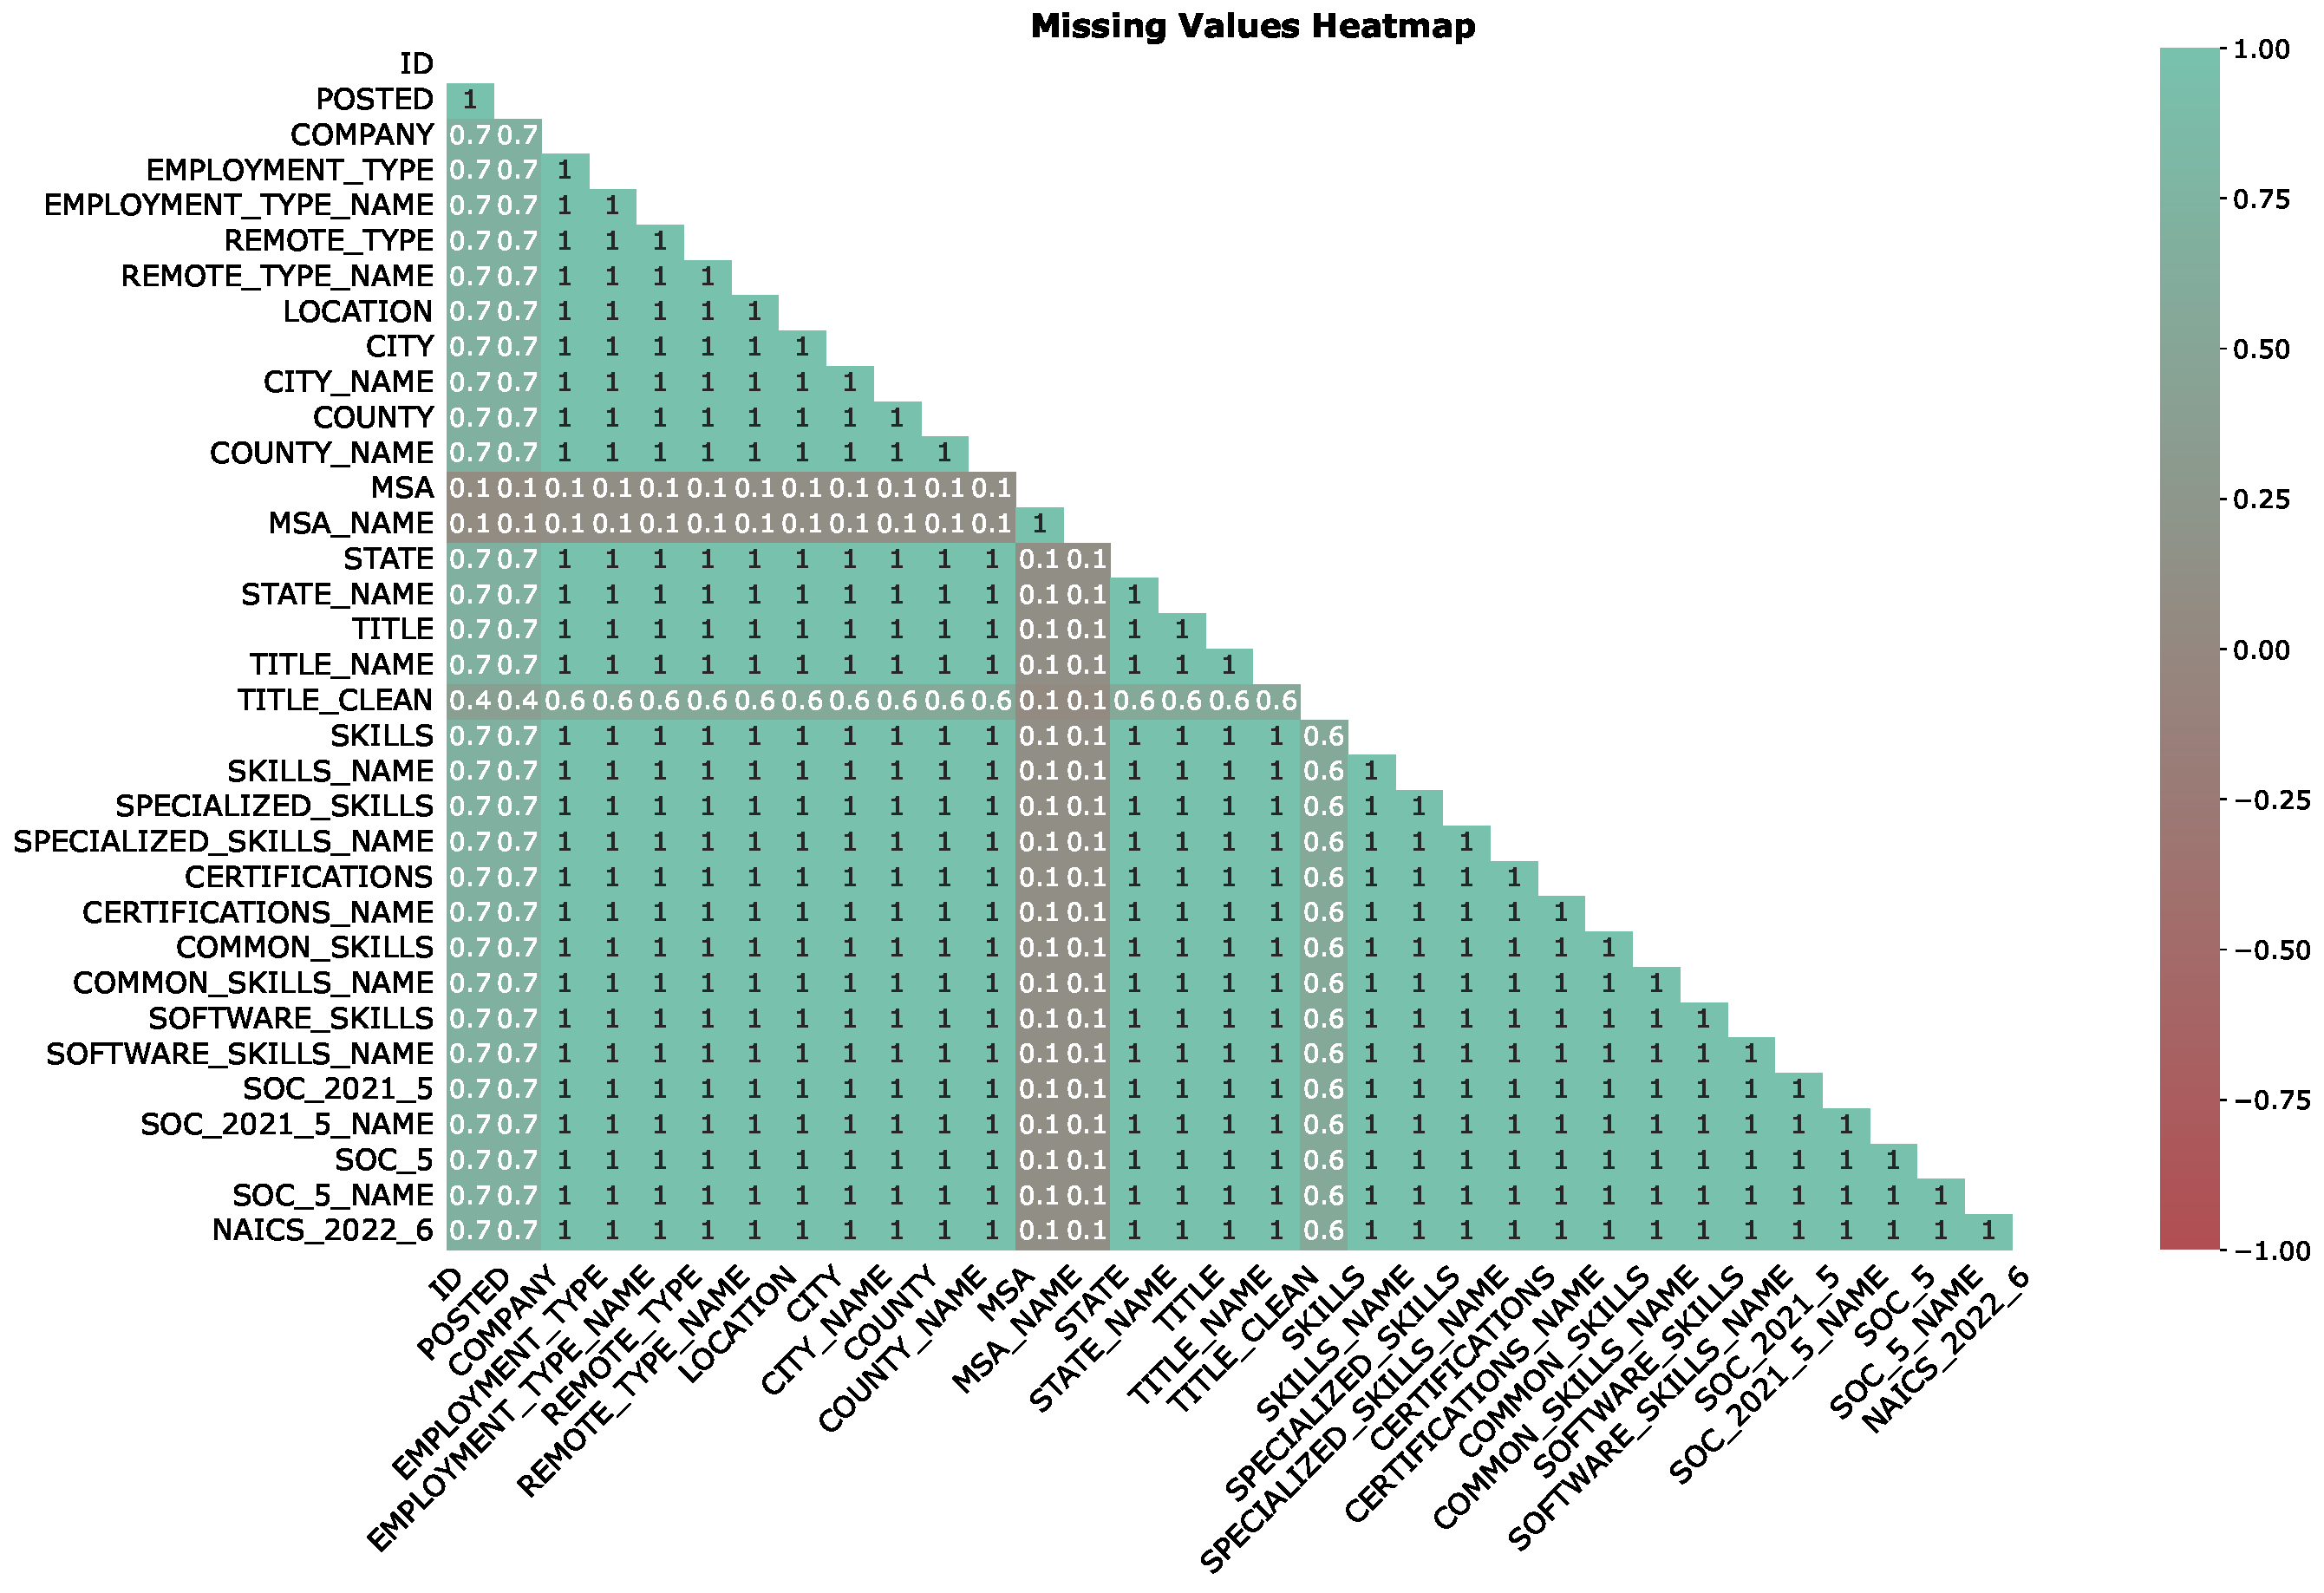
\includegraphics[keepaspectratio]{data_analysis_files/figure-pdf/cell-5-output-2.pdf}}

The heatmap shows a few missing values in the dataset. In this dataset
most fields cluster near 1. The value 1 (dark blue) means the two
columns have missing values together. 0.0 value (white) suggest there is
no relationship.

\subsection{Remove Duplicates}\label{remove-duplicates}

\begin{Shaded}
\begin{Highlighting}[]
\NormalTok{data }\OperatorTok{=}\NormalTok{ data.drop\_duplicates(subset}\OperatorTok{=}\NormalTok{[}\StringTok{"TITLE"}\NormalTok{, }\StringTok{"COMPANY"}\NormalTok{, }\StringTok{"LOCATION"}\NormalTok{, }\StringTok{"POSTED"}\NormalTok{], keep}\OperatorTok{=}\StringTok{"first"}\NormalTok{)}
\end{Highlighting}
\end{Shaded}

\subsection{Job Postings by Industry}\label{job-postings-by-industry}

\begin{Shaded}
\begin{Highlighting}[]
\NormalTok{data[}\StringTok{"posting\_count"}\NormalTok{] }\OperatorTok{=}\NormalTok{ data[}\StringTok{"ID"}\NormalTok{]. groupby(data[}\StringTok{"INDUSTRY"}\NormalTok{]).transform(}\StringTok{"count"}\NormalTok{)}

\NormalTok{industry\_summary }\OperatorTok{=}\NormalTok{ data.groupby(}\StringTok{"INDUSTRY"}\NormalTok{)[}\StringTok{"posting\_count"}\NormalTok{].first().sort\_values(ascending}\OperatorTok{=}\VariableTok{False}\NormalTok{).head(}\DecValTok{25}\NormalTok{)}

\ImportTok{import}\NormalTok{ seaborn }\ImportTok{as}\NormalTok{ sns}
\ImportTok{import}\NormalTok{ matplotlib.pyplot }\ImportTok{as}\NormalTok{ plt}

\NormalTok{plt.figure(figsize}\OperatorTok{=}\NormalTok{(}\DecValTok{12}\NormalTok{, }\DecValTok{10}\NormalTok{))}
\NormalTok{sns.barplot(x}\OperatorTok{=}\NormalTok{industry\_summary.values, y}\OperatorTok{=}\NormalTok{industry\_summary.index, orient}\OperatorTok{=}\StringTok{\textquotesingle{}h\textquotesingle{}}\NormalTok{)}
\NormalTok{plt.title(}\StringTok{"Top 25 Job Postings by Industry"}\NormalTok{, fontsize}\OperatorTok{=}\DecValTok{16}\NormalTok{, pad}\OperatorTok{=}\DecValTok{20}\NormalTok{)}
\NormalTok{plt.xlabel(}\StringTok{"Number of Job Postings"}\NormalTok{, fontsize}\OperatorTok{=}\DecValTok{12}\NormalTok{)}
\NormalTok{plt.ylabel(}\StringTok{"Industry"}\NormalTok{, fontsize}\OperatorTok{=}\DecValTok{12}\NormalTok{)}
\NormalTok{plt.tight\_layout()}
\NormalTok{plt.show()}
\end{Highlighting}
\end{Shaded}

\pandocbounded{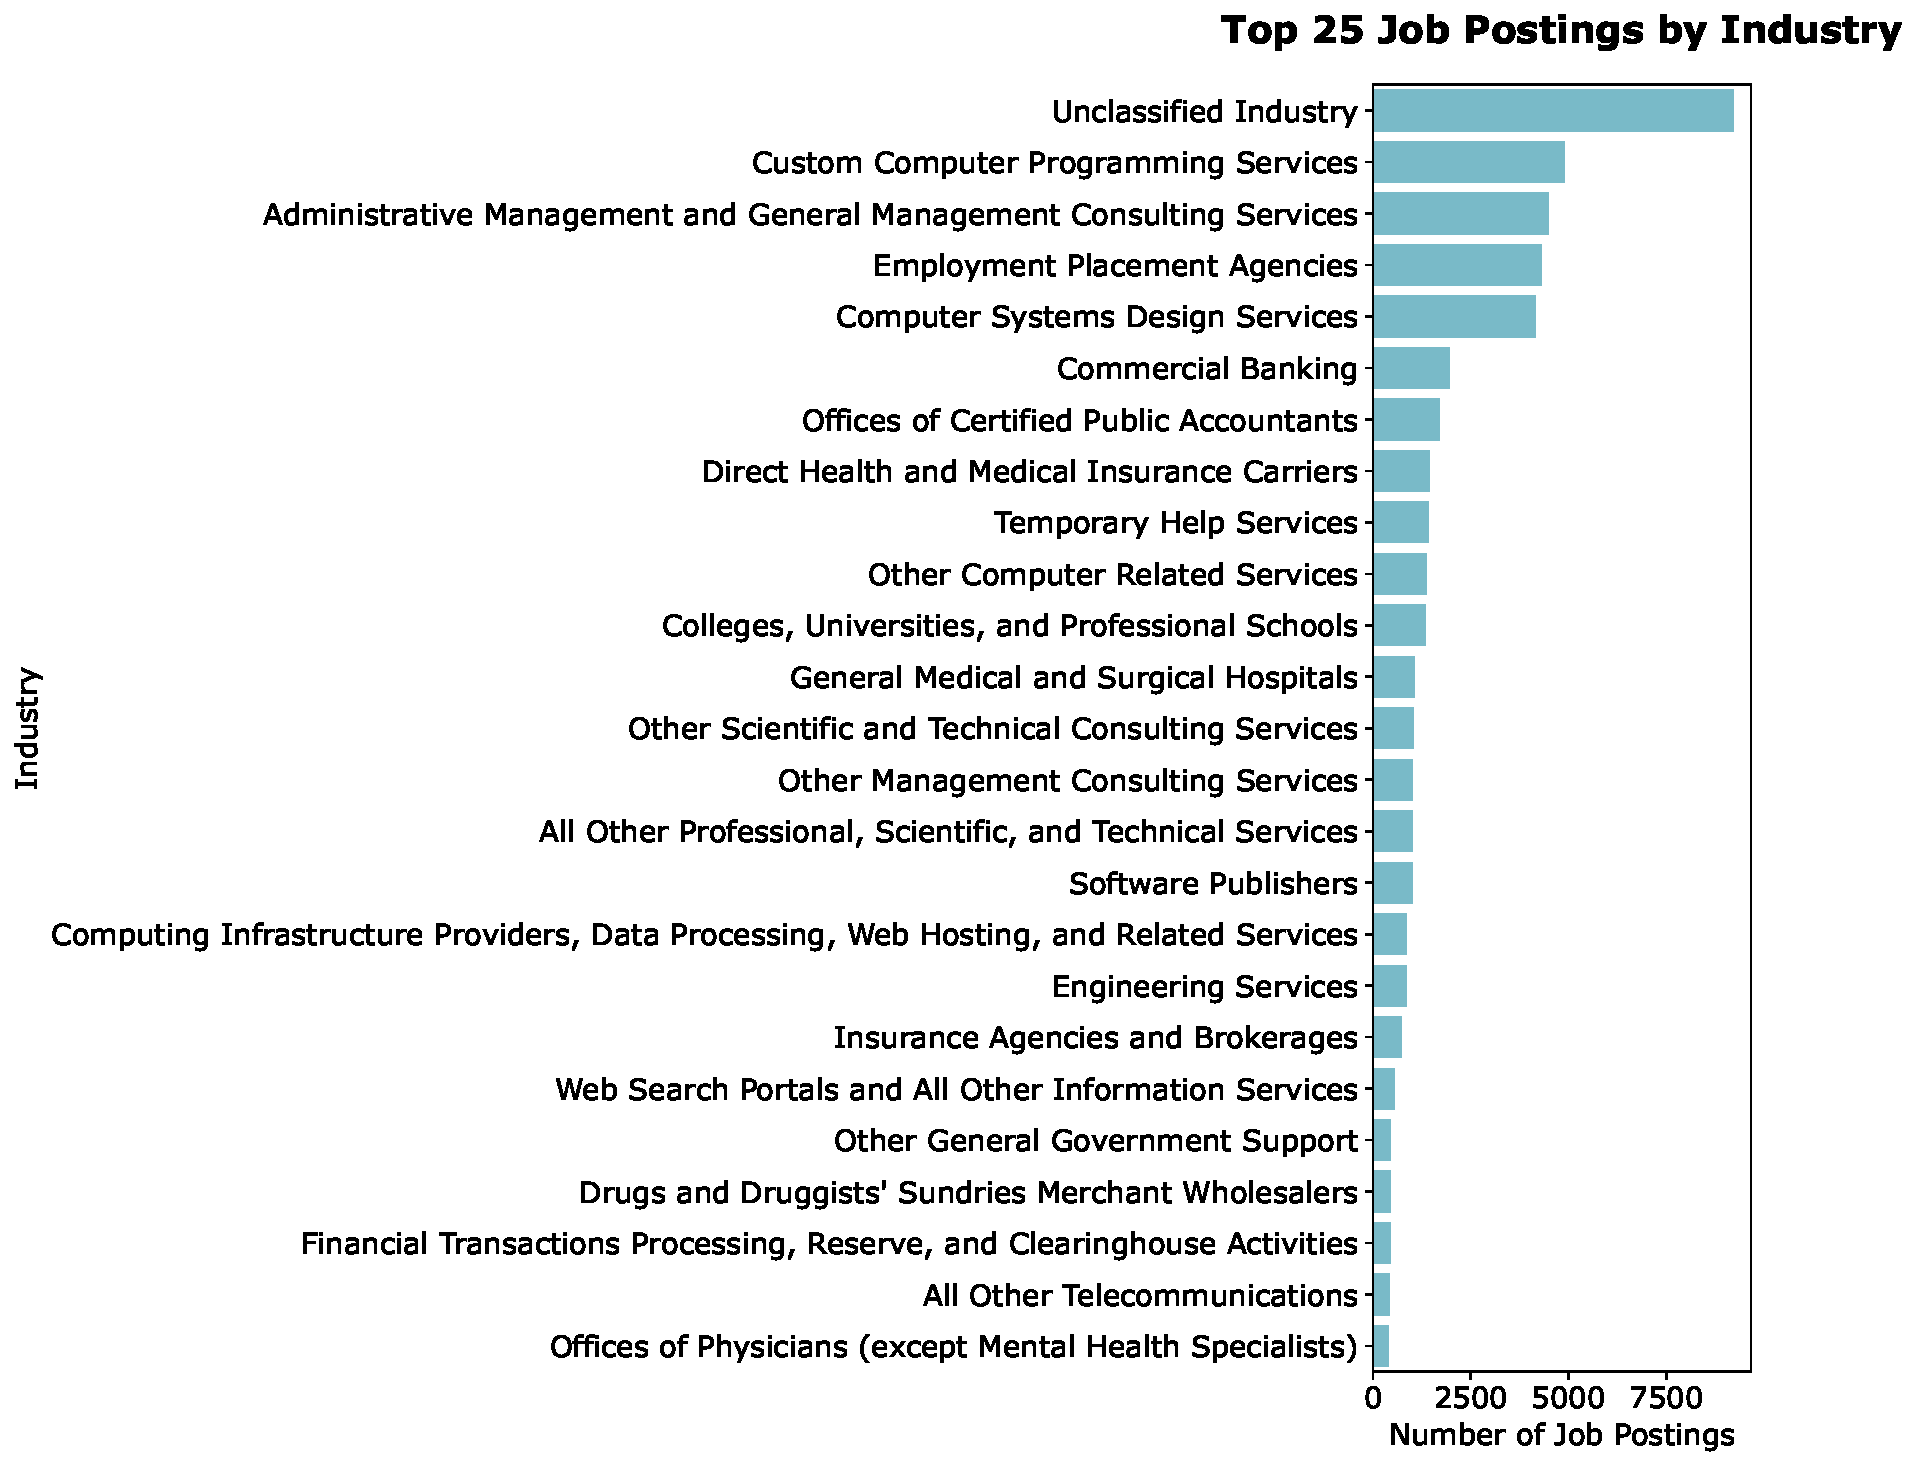
\includegraphics[keepaspectratio]{data_analysis_files/figure-pdf/cell-7-output-1.pdf}}

\subsection{Salary Distribution by
Industry}\label{salary-distribution-by-industry}

\begin{Shaded}
\begin{Highlighting}[]
\NormalTok{data[}\StringTok{"AVERAGE\_INDUSTRY\_SALARY"}\NormalTok{] }\OperatorTok{=}\NormalTok{ data[}\StringTok{"SALARY"}\NormalTok{]. groupby(data[}\StringTok{"INDUSTRY"}\NormalTok{]).transform(}\StringTok{"mean"}\NormalTok{).}\BuiltInTok{round}\NormalTok{()}

\NormalTok{top\_40\_industries }\OperatorTok{=}\NormalTok{ data.groupby(}\StringTok{"INDUSTRY"}\NormalTok{)[}\StringTok{"AVERAGE\_INDUSTRY\_SALARY"}\NormalTok{].first().sort\_values(ascending}\OperatorTok{=}\VariableTok{False}\NormalTok{).head(}\DecValTok{40}\NormalTok{).index}
\NormalTok{filtered\_data }\OperatorTok{=}\NormalTok{ data[data[}\StringTok{"INDUSTRY"}\NormalTok{].isin(top\_40\_industries)]}

\NormalTok{plt.figure(figsize}\OperatorTok{=}\NormalTok{(}\DecValTok{20}\NormalTok{, }\DecValTok{10}\NormalTok{))}
\NormalTok{sns.boxplot(data}\OperatorTok{=}\NormalTok{filtered\_data, x}\OperatorTok{=}\StringTok{"INDUSTRY"}\NormalTok{, y}\OperatorTok{=}\StringTok{"SALARY"}\NormalTok{, }
\NormalTok{            order}\OperatorTok{=}\NormalTok{top\_40\_industries)}
\NormalTok{plt.title(}\StringTok{"Salary Distribution by Industry (Top 40 by Average Salary)"}\NormalTok{, fontsize}\OperatorTok{=}\DecValTok{16}\NormalTok{, pad}\OperatorTok{=}\DecValTok{20}\NormalTok{)}
\NormalTok{plt.xlabel(}\StringTok{"Industry"}\NormalTok{, fontsize}\OperatorTok{=}\DecValTok{12}\NormalTok{)}
\NormalTok{plt.ylabel(}\StringTok{"Salary"}\NormalTok{, fontsize}\OperatorTok{=}\DecValTok{12}\NormalTok{)}
\NormalTok{plt.xticks(rotation}\OperatorTok{=}\DecValTok{45}\NormalTok{, ha}\OperatorTok{=}\StringTok{\textquotesingle{}right\textquotesingle{}}\NormalTok{)}
\NormalTok{plt.tight\_layout()}
\NormalTok{plt.show()}
\end{Highlighting}
\end{Shaded}

\pandocbounded{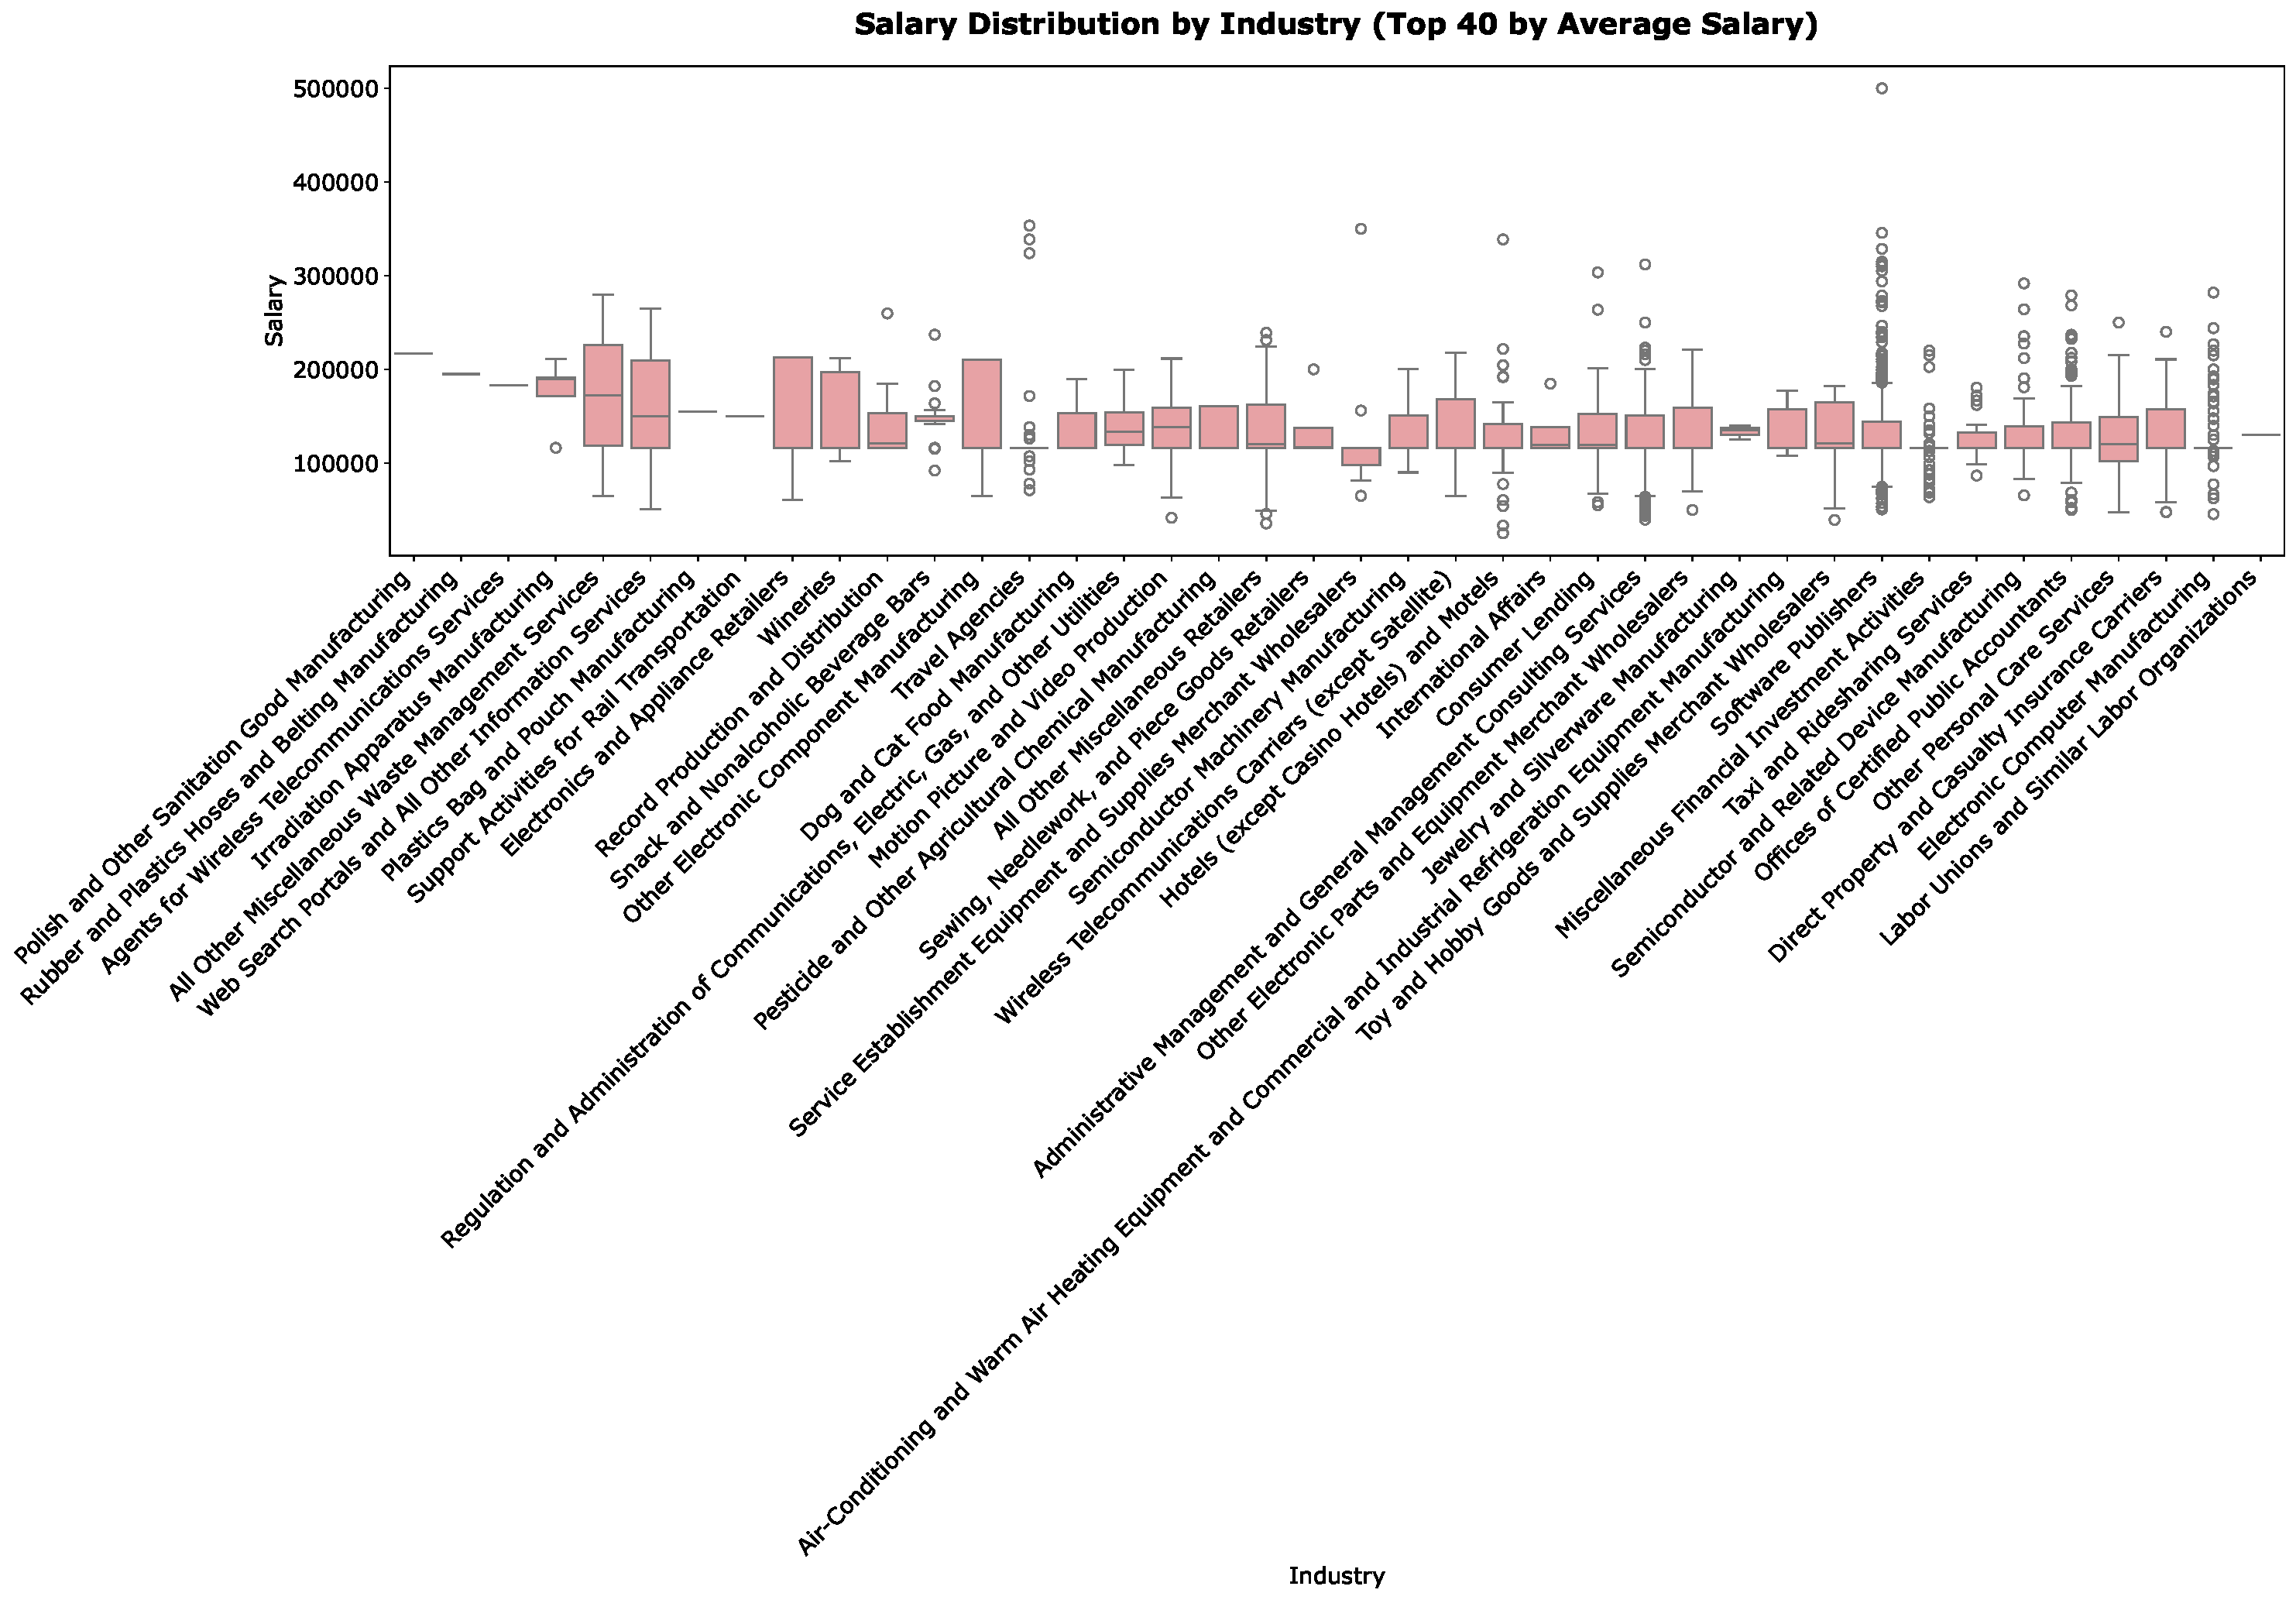
\includegraphics[keepaspectratio]{data_analysis_files/figure-pdf/cell-8-output-1.pdf}}

\subsection{Remote vs.~On-Site Jobs}\label{remote-vs.-on-site-jobs}

\begin{Shaded}
\begin{Highlighting}[]
\NormalTok{remote\_counts }\OperatorTok{=}\NormalTok{ data[}\StringTok{"REMOTE\_TYPE\_NAME"}\NormalTok{].value\_counts()}

\NormalTok{plt.figure(figsize}\OperatorTok{=}\NormalTok{(}\DecValTok{8}\NormalTok{, }\DecValTok{8}\NormalTok{))}
\NormalTok{plt.pie(remote\_counts.values, labels}\OperatorTok{=}\NormalTok{remote\_counts.index, autopct}\OperatorTok{=}\StringTok{\textquotesingle{}}\SpecialCharTok{\%1.1f\%\%}\StringTok{\textquotesingle{}}\NormalTok{)}
\NormalTok{plt.title(}\StringTok{"Remote vs. On{-}Site Jobs"}\NormalTok{, fontsize}\OperatorTok{=}\DecValTok{16}\NormalTok{, pad}\OperatorTok{=}\DecValTok{20}\NormalTok{)}
\NormalTok{plt.show()}
\end{Highlighting}
\end{Shaded}

\pandocbounded{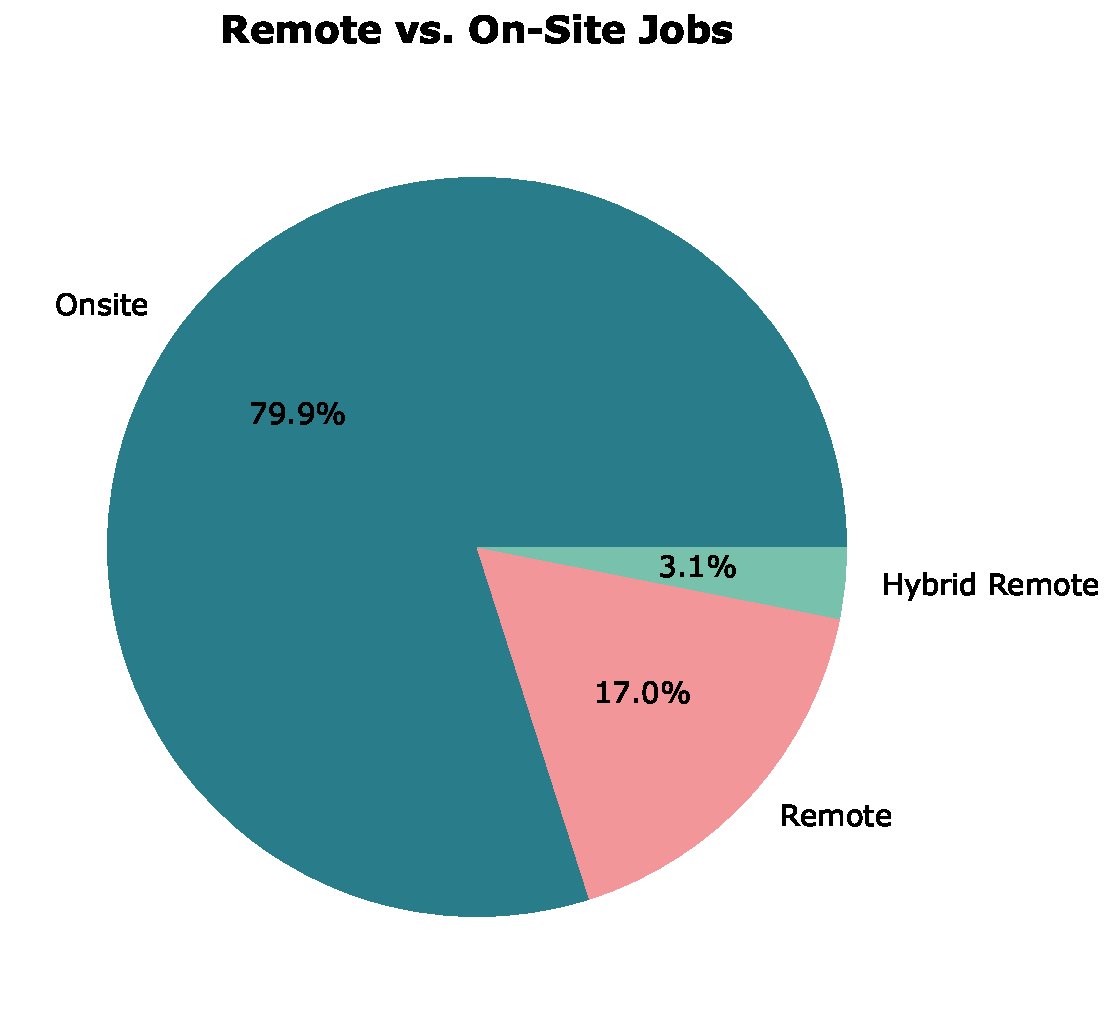
\includegraphics[keepaspectratio]{data_analysis_files/figure-pdf/cell-9-output-1.pdf}}

\subsection{Why these visualizations were
chosen}\label{why-these-visualizations-were-chosen}

\begin{itemize}
\tightlist
\item
  \textbf{Bar Chart: Job Postings by Industry}

  \begin{itemize}
  \tightlist
  \item
    Makes it easy to compare job postings across different industries.\\
  \item
    Provides a clear ranking that is simple to interpret.
  \end{itemize}
\item
  \textbf{Boxplot: Salary Distribution by Industry}

  \begin{itemize}
  \tightlist
  \item
    Shows medians, outliers, and summarizes salary distributions.\\
  \item
    Allows for comparisons between industries and helps detect salary
    variability.
  \end{itemize}
\item
  \textbf{Pie Chart: Job Location Types}

  \begin{itemize}
  \tightlist
  \item
    Provides a clear visual breakdown of remote versus on-site jobs
    within the dataset.
  \end{itemize}
\end{itemize}

\subsection{Key insights from each
graph}\label{key-insights-from-each-graph}

\begin{itemize}
\tightlist
\item
  \textbf{Bar Chart: Top 25 Industries by Job-Posting Volume}

  \begin{itemize}
  \tightlist
  \item
    The distribution is skewed, showing demand concentrated in
    technology and professional services.\\
  \item
    A large portion of ``unclassified industry'' job postings suggests
    many jobs are not mapped to any industry.
  \end{itemize}
\item
  \textbf{Boxplot: Salary Distribution by Industry}

  \begin{itemize}
  \tightlist
  \item
    Salaries across the 40 industries skew high, with medians generally
    in the \$120k--\$170k range.\\
  \item
    Industries with higher medians and greater dispersions include
    software/semiconductors and consulting.\\
  \item
    Several industries have wide IQRs and many upper outliers, while
    some have less variability, indicating standardized pay.
  \end{itemize}
\item
  \textbf{Pie Chart: Job Location Types}

  \begin{itemize}
  \tightlist
  \item
    17\% of jobs are remote, 3.1\% are hybrid, and 1.6\% are not
    remote.\\
  \item
    A large number of job postings do not specify whether the job is
    remote or on-site.
  \end{itemize}
\end{itemize}




\end{document}
